\subsection{Galaxy formation}

\subsubsection{Dark matter halos}
The $\Lambda$CDM model for our universe gives a bottom-up solution to galaxy formation. Essentially this means that larger galaxies have formed through mergers of smaller galaxies. In the early universe, dark matter is distributed isotropically on large scales, but with local perturbations. These perturbations in the density field grow with time, and the dark matter collapses into clumps known as halos. The halos provide the initial gravitational well needed for baryonic matter to collapse and create stars. This leads to galaxies forming at the center of their respective halos. Gravitationally bound halos are called subhalos, and are part of a larger host halo. Subhalos will fall towards the central subhalo, and accrete onto it, depending on variables like the subhalos size and orbit. There may be subhalos without an attached galaxy, but all galaxies have a dark matter subhalo.

\subsubsection{Stellar-to-Halo mass relation}
The stellar-to-halo mass relation (SHMR) gives us an idea about what size galaxy populates a dark matter halo of a certain size. One way of looking for this relation is through a method called abundance matching \parencite{None2000}. Abundance matching is a numerical method which employs a guess for the form of a relation to simulate how such a universe might look, and then compares it to observations. By tweaking the form of the equation, a better match can be achieved, and as such a better estimate for the right answer. 

Using abundance matching, the SHMR has been found to be well described by a power law for low-mass galaxies, and a subpower law for the high-mass end of the spectrum \parencite{Behroozi2013}. 

\begin{equation}
    \log_{10}(M_*(M_h)) = \log_{10}(\epsilon M_1) + f(\log_{10}(M_h/M_1)) -f(0),
\end{equation}
\begin{equation*}
    f(x) = -\log_{10}(10^{\alpha x}+1)+\delta \frac{(\log_{10}(1+\exp(x)))^\gamma}{1 +\exp(10^{-x})}
\end{equation*}

Here $M_*$ is the stellar mass, $M_h$ is the halo mass, $M_1$ is a characteristic halo mass, $\delta$ is the strength of the subpower law, $\alpha$ is the power law slope for $M_h << M_1$ and $\gamma$ is the power law index for $M_h >> M_1$.

This gives us a relation that matches smaller halos to smaller galaxies, and vice versa, as well as a characteristic halo mass of about $10^{12}M_{\odot}$.

\subsection{Galaxy evolution and classification}
As soon as telescopes became good enough to clearly make out galaxies in the sky, it became apparent that galaxies come in many different shapes and sizes. The morphology of a galaxy is important, because it turns out that morphology is closely linked to other properties of the galaxy. Edwin Hubble classified galaxies on a spectra \parencite{Hubble1926}, with spiral galaxies (galaxies with a prominent disk component) on one end of the spectrum and elliptical galaxies (galaxies that have a dominant spheroidal component) on the other (see Figure \ref{hubble}). He thought that galaxies started off as ellipticals and evolved along the spectrum, becoming more disk-dominated as it aged. This is the reason that elliptical and spiral galaxies are known as early and late type galaxies. These terms can be confusing as it turns out that Hubble was probably wrong, and the evolution of galaxies probably moves in the other direction. 

In the $\Lambda$CDM model, galaxies grow through mergers. Mergers are separated into two types, major and minor mergers.  Major mergers are events where two galaxies of equal size collide and become one galaxy. Simulations have shown that a major merger between two disk galaxies produces an elliptical. The Milky Way, which is a large spiral galaxy ($M_*>10^{10}$) has probably grown through many smaller minor mergers, and thus kept its disky part.

\begin{figure}
    \centering
    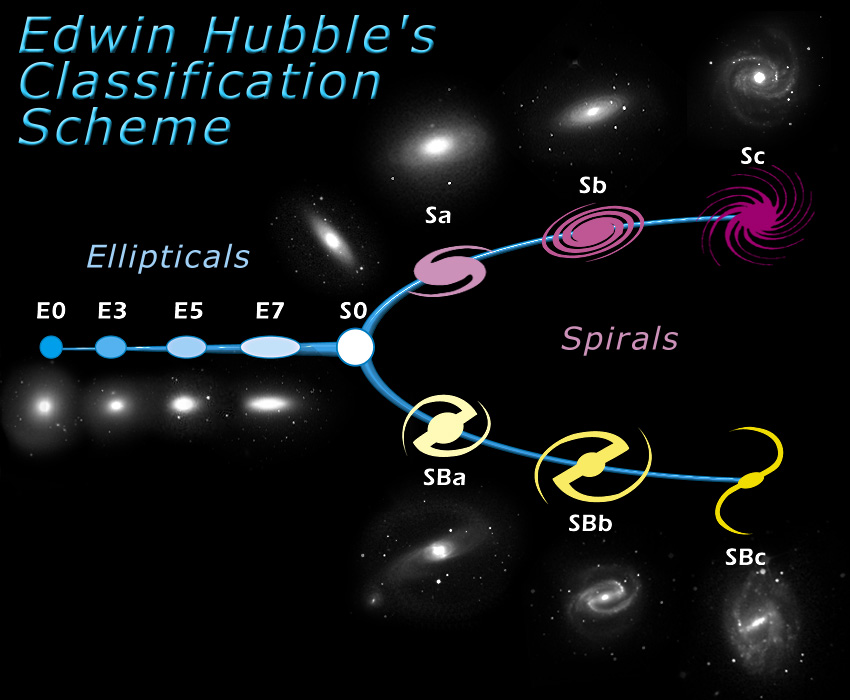
\includegraphics[width=0.5\textwidth]{images/hubble.jpg}
    \caption{Chart from 1999 showing the original classifications of galaxy morphology. Credit: ESA/Hubble}
    \label{hubble}
\end{figure}

It is not always easy to distinguish between a disky elliptical and a spiral with a large spheroidal component (bulge). Some galaxies are in the middle of a merging process. These can have very irregular shapes, and so are hard to classify. Other galaxies are very small, so called dwarf galaxies. These galaxies tend to have very little stellar mass compared to dark matter, so they do not exhibit the properties of ellipticals, even though they may be more elliptical in shape. In this project, we mostly look at larger, central galaxies, so we will not have to consider most of these special galaxy types.

\subsubsection{Elliptical (early type) galaxies}
Elliptical galaxies are mainly pressure-dominated systems, meaning that the motion of the stars is predominantly radial. The largest galaxies in the universe tend to be ellipticals, but they come in all sizes. The star population of ellipticals is generally older than that of spirals, and there is usually little to no star formation. There is very little gas and dust in ellipticals, and they tend to emit more light in the redder end of the EM spectrum. Early type galaxies are less common than late type galaxies, and are more usually found in galaxy clusters.

\subsubsection{Spiral (late type) galaxies}
Late type galaxies have a prominent disky component, orbiting around the galaxy's center. The rotational velocity of the disk is typically much larger than the velocity dispersion of the galaxy's bulge. The stars in a spiral galaxy are usually much younger than those in early types. There is a lot of gas and dust present in spirals, giving rise to ongoing star formation. Late type galaxies are bluer in color than early types. Field galaxies, galaxies that are not part of a galaxy cluster, are predominantly spirals. 

The large rotational velocities of the disky part of late-type galaxies perplexed early astrophysicists, as the mass inferred by the rotational motion was much greater than that which could be accounted for by the stars and gas in the galaxy. An effort to solve this problem led to the theory of dark matter, and later to the $\Lambda$CDM model.


\subsection{Galaxy properties}


\subsubsection{The Tully-Fisher relation}

In 1977, R.B. Tully and J.R. Fisher \parencite{TullyFisher1977} published a paper where they found a surprisingly good correlation between the luminosity of a spiral galaxy and the rotational speed of its disk on the form of a simple power law with index 4.

\begin{equation}
    L \propto v_{rot}^4 
\end{equation}

As stellar mass is directly proportional to the luminosity, this gives us the ability to estimate stellar mass from a simple measurement of the rotational velocity.

\begin{equation}
    M_* \propto v_{rot}^4 
\end{equation}

This relation is a great tool for estimating the distance (and hence age) to a galaxy, as the calculated luminosity can be compared to the observed luminosity at Earth. For numerical simulations, being able to reproduce the Tully-Fisher relation is an essential way to check if the model used is reliable.

\subsubsection{The Faber-Jackson relation and the Fundamental Plane}
At around the same time that Tully and Fisher published their paper, Sandra M. Faber and Robert Earl Jackson published a paper that linked the velocity dispersion and luminosity of early-type galaxies. The proposed relation was on the form of a power law as well, with an index of approximately 4 \parencite{FaberJackson1976}.

\begin{equation}
    L \propto \sigma^{\gamma} 
\end{equation}

This is known as the Faber-Jackson (FJ) relation. The correlation was not as tight as the Tully-Fisher relation however, and it was later found that the velocity dispersion also was dependent on the size of the galaxy.

\begin{equation}
    \sigma \propto L^a R^b
\end{equation}

With the radius added into the equation, the deviations from observations became much less significant. Most ellipticals are found on the same plane in ${\sigma, R, L}$ space. This plane became known as the Fundamental Plane (FP), through a paper published in 1987 \parencite{Djorgovski1987}, and is also something which successfull numerical simulations must reproduce.

\subsubsection{Color bimodality}
Color, in astrophysics, is defined as the difference in magnitudes measured for a galaxy by two different optical filters. A galaxy that is "blue" has a larger amount of blue light than red. In general, galaxies are found to inhabit one of two groups on a color-mass diagram, blue and red. The blue galaxies are most often late type galaxies, while the red ones are mainly ellipticals. There are many factors that contribute to the color of a galaxy, like stellar age and metallicity as well as the amount of gas the light has passed through and its metallicity.

\subsubsection{Supermassive Black Holes}
Almost every large galaxy with a spheroidal component has a supermassive black hole (SMBH) in its center. These are black holes with masses over $10^6 M_{\odot}$ and even above $10^9 M_{\odot}$. The mass of the SMBH correlates surprisingly well with other properties of the galaxy, such as the velocity dispersion and luminosity. This is surprising because the SMBH only has a gravitational influence within a pretty small radius compared to the entire galaxy, which suggests that the SMBH evolves along with the galaxy and that their formation is linked. In fact, it seems very likely that these gigantic black holes play a vital role in galaxy evolution, and are a central component of the galaxy as a whole.